\documentclass[11pt]{article}

\usepackage{amssymb}
\usepackage{amsthm}
\usepackage{amsmath}
\usepackage[table]{xcolor}
\usepackage{enumitem}
\usepackage{multirow}
\usepackage{hyperref}
\usepackage{graphicx}
\hypersetup{
  colorlinks, urlcolor = blue
}

\usepackage{array}
\newcolumntype{L}[1]{>{\raggedright\let\newline\\\arraybackslash\hspace{0pt}}m{#1}}
\newcolumntype{C}[1]{>{\centering\let\newline\\\arraybackslash\hspace{0pt}}m{#1}}
\newcolumntype{R}[1]{>{\raggedleft\let\newline\\\arraybackslash\hspace{0pt}}m{#1}}


\begin{document}

\title{\endgraf\rule{\textwidth}{.4pt}\\Auto Encoder No 2}
\author{David Ishak Kosasih (20195033)}
\date{\today\endgraf\rule{\textwidth}{.4pt}}
\maketitle

\begin{enumerate}
\setcounter{enumi}{0}

%%%%%%%%%%%%%%%%%%%%%%%%%%%%%%%%%%%%%%%%%%%%%%%%%%%%%%%%%%%%%%%%%%%%
%% number 1
\item Experiment result for MNIST dataset:
	% explenation	
	\begin{figure}[ht]
		\centering
		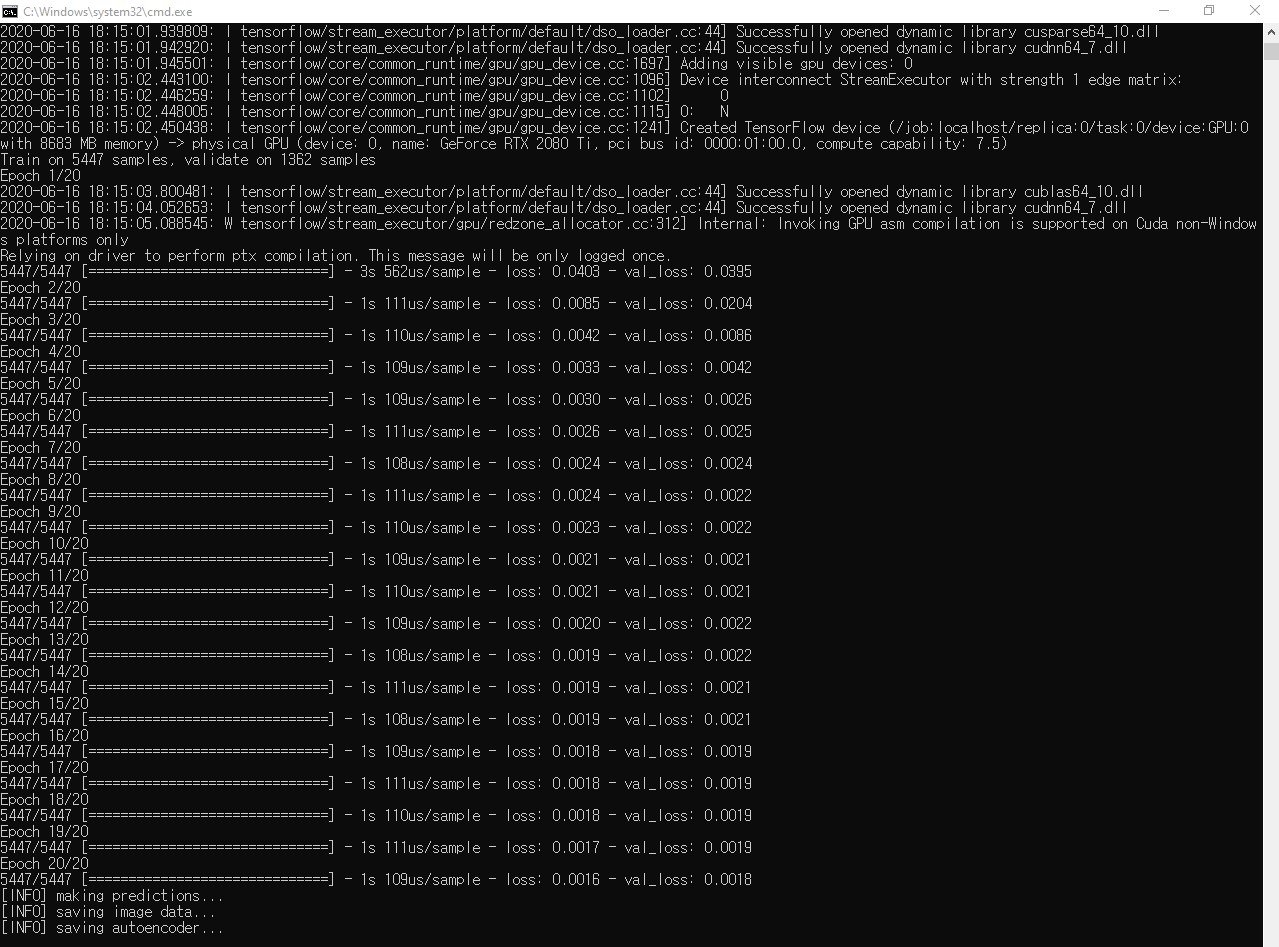
\includegraphics[width=0.7\linewidth]{Images/run_cmd}
		\caption{Train history in Command Prompt (CMD)}
		\label{fig:run_cmd}
	\end{figure}

	\begin{description}[style=unboxed,leftmargin=0.2cm]
		\item In Fig. \ref{fig:run_cmd}, we can see the training history over 20 epoch. The final loss and validation loss are 0.0016 and 0.0018 respectively. The entire decrease in the MSE error can be seen in Fig. \ref{fig:Loss Plot}. 
	\end{description}
	
	\begin{figure}[ht]
		\centering
		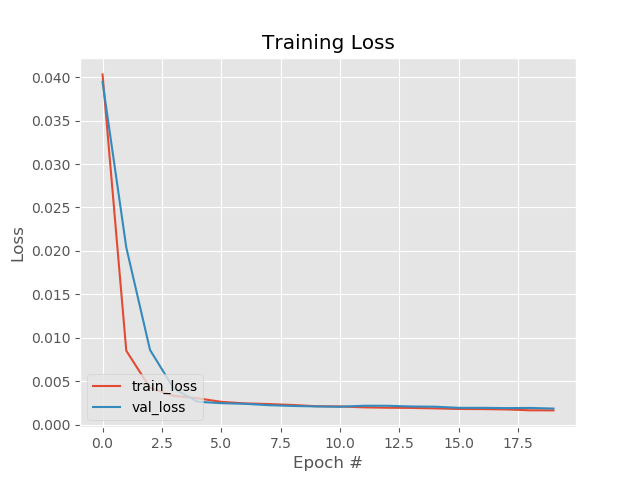
\includegraphics[width=0.7\linewidth]{Images/plot}
		\caption{In this plot we can see the loss curves}
		\label{fig:Loss Plot}
	\end{figure}

	\begin{description}[style=unboxed,leftmargin=0.2cm]
		\item As we can see from Fig. \ref{fig:Loss Plot}, our MSE error between original input images and reconstructions plummeted in the first five epoch before making a steady progress until it reached 0.0016 and 0.0018 for loss and validation loss respectively in the last epoch. As stated in the author's documentation, the encoder accepts input data and compresses it into the latent-space representation while the decoder attempts to reconstruct input data from the latent space. If we use MSE as our loss function to minimize the difference between original and reconstructed images, then we will obviously get this result. Low MSE loss indicates that our model can successfully reconstruct the original image. 
	\end{description}
	
	\begin{figure}[ht]
		\centering
		
\includegraphics[width=0.15\linewidth]{Images/recon_vis}
		\caption{Reconstruction result of MNIST dataset}
		\label{fig:recon_vis}
	\end{figure}
	
	\begin{description}[style=unboxed,leftmargin=0.2cm]
		\item Fig. \ref{fig:recon_vis} depicts the reconstructed MNIST dataset. It could successfully learn to correctly reconstruct the 1 digit from MNIST dataset. Autoencoder.model and images.pickle files can also be found in this github URL : \url{https://github.com/ishakdavidk/Deep-Learning/tree/master/Homework\%206/No\%202}
	\end{description}	

\end{enumerate}

\end{document}